\mychapter{System Design}{System Design}{}\label{chap:sys-design}

\begin{figure}[H]
    \centering
    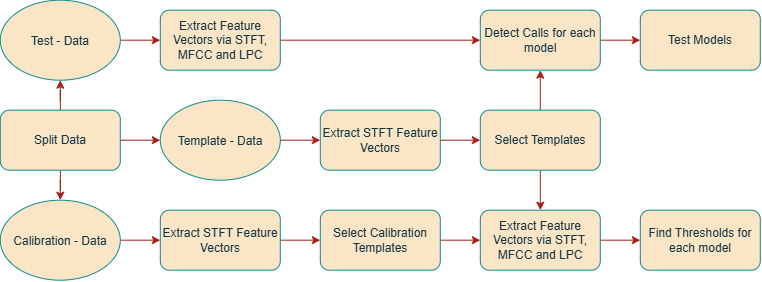
\includegraphics[width=0.8\linewidth]{figures/Skrip_CH3.drawio.png}
    \caption{Zoomed out image of System Design}\label{fig:systen-design}
\end{figure}


\mysection{Overview}{Overview}\label{sec:overview}
The project was coded in Python. The functionality of each section of the project was placed in relevant .py files which were imported to the relevant jupyter notebook which was used for that section.

\mysection{Feature Extraction Methods}{Feature Extraction Methods}\label{sec:feature-extraction-methods}
The raw audio recorded by the hydrophone was stored in .wav files with a sampling frequency of 8kHz. Before extracting feature vectors from audio segments the audio was first downsampled to 1kHz sampling rate. This helped remove unecessary frequency 
information as the Nyquist Frequncy ($f_s/2$) for a 1kHz sampling rate is 500 Hz.\cite{nyq}

Most of the Bryde's Whale vocalizations occur below 200 Hz. Thus, this sampling rate also ensures no relevant information was lost before analysis.\cite{bryde_whales_SA} 

\mysubsection{STFT}{STFT}\label{sec:stft}
The signal.stft function from the scipy library was used to calculate the STFT magnitudes for use as feature vectors. 
Window length $L$, as referenced in Eq.\eqref{eq:freq_resolution}, is calculated by multiplying $f_s$, the sampling frequency of the given audio segment, with the chosen STFT frame duration. No set frame duration was selected as the optimal 
frame duration was chosen during the calibration stage of this project.
The window ovelrap $H$, as referenced in Eq.\eqref{eq:freq_resolution}, is calculed by multiplying $f_s$ with the chosen overlap percentage. For this project the overlap percentage was chosen as 0,75. The high overlap percentage produced a 
smooth spectrogram when viewing the time-frequency representation of the given audio segment.
A Hamming window was chosen to decrease any spectral leakage caused by the finite length of the windows used to extract the feature vectors.\cite{stft_kamper}\cite{hamm}

\mysubsection{MFCC}{MFCC}\label{sec:mfcc}
used librosa

\mysubsection{LPC}{LPC}\label{sec:lpc}

\mysection{DTW methodology}{DTW methodology}\label{sec:dtw_method}
used librosa. Calculated the cost matrix of a large stream of audio against a template. Only used the bottom rows costs since these show dips when a call is detected as the cost bottoms out.
A call was detected by determining where the dips were and then finding whether the end cost of that dip was below the threshold.
\mysection{Hyperparameter Tuning}{Hyperparameter Tuning}\label{sec:hyperparameter-tuning}
The frame length of any feature extraction method affects the frequency resolution. Therefore, different widths of frame length (0.048, 0.064, 0.096, 0.128, 0.192, 0.256, 0.384, 0.512) were tested to see 
which produced the best F1 score. In the process of determining the best frame length the F1 score is calculated by also finding the best possible thresholds for which each call can be seperated as either 
a call or background noise. While the project only focused on general detection of calls and not on classification, three different thresholds, one for each call type, were calculated and used. The reason for this 
is that choosing one overarching threshold would make the model far too lenient for some calls as call types such as single-tones and burst-tonals tend to have a significant difference in threshold choice. 
Even though three different thresholds were chosen based on the templates from each call type in the final detection only general call detection was considered and not whether the model classified the calls 
correctly. This was due to the fact that single0tones and multi-tones sometimes look very similar and thus tend to be incorrectly classified.

When deciding whether an audio segment is a call or not that segment is compared against all 30 templates (10 for each call type). For each call type some of the 10 templates will say that it is a call and others will say that it 
is not since the templates were chosen for varying noise conditions. The vote fraction is used to decide whether the audio segment is from that call type or not. If that vote fraction amount of the 10 calls say it is a call then 
it will be classified as such if less than that vote fraction agree that it is a call then it will not be classified as a call. The F1 score is calculated using different voting fractions (0.1, 0.2, 0.3, 0.4, 0.5, 0.6, 0.7, 0.8, 0.9, 1.0) 
as well as the chosen frame length and thresholds. This F1 is used to choose the best possible voting fraction for all three call types. 
\mysection{Training Procedure}{Training Procedure}\label{sec:training-procedure}

\mysection{Evaluation Metrics}{Evaluation Metrics}\label{sec:evaluation-metrics}